\documentclass[specialist,
substylefile = spbu.rtx,
               subf,href,colorlinks=true, 12pt]{disser}

\usepackage[a4paper,
            mag=1000, includefoot,
            left=3cm, right=1.5cm, top=2cm, bottom=2cm, headsep=1cm, footskip=1cm]{geometry}
\usepackage[T2A]{fontenc}
\usepackage[utf8]{inputenc}
%\usepackage[cp1251]{inputenc}
\usepackage[english,russian]{babel}
\ifpdf\usepackage{epstopdf}\fi

% Точка с запятой в качестве разделителя между номерами цитирований
%\setcitestyle{semicolon}

% Использовать полужирное начертание для векторов
\let\vec=\mathbf

% Включать подсекции в оглавление
\setcounter{tocdepth}{2}


%----------------------------------------------------------------
%\usepackage{refcheck}
\usepackage{indentfirst}
\usepackage{amsmath}
\usepackage{amssymb}
\usepackage{amsthm}
\usepackage{graphicx}
\graphicspath{{images/}}
\usepackage{wrapfig}
\usepackage{listings}
\usepackage{ mathrsfs }
%\usepackage{subfigure}
\newtheorem{proporsal}{Предложение}
\newtheorem{definition}{Определение}
\newtheorem{remark}{Замечание}
\newtheorem{statement}{Утверждение}
\newtheorem*{consequence}{Следствие}
\newcounter{algorithm}
\newcounter{algorithm2}
\DeclareMathOperator*{\longrightarrowt}{\longrightarrow}
\DeclareMathOperator*{\tot}{\to}


\begin{document}

%
% Титульный лист на русском языке
%

%-------------------------------------
%% Название организации
%\institution{%
%    Правительство Российской Федерации \\
%    Федеральное государственное автономное образовательное учреждение \\
%    высшего профессионального образования \\
%    <<Национальный исследовательский университет \\
%    <<Высшая школа экономики>> \\
%    Факультет компьютерных наук
%}
%% Имя лица, допускающего к защите (зав. кафедрой)
%
%\title{Бакалаврская работа}
%
%% Тема
%\topic{\normalfont\scshape%
%   Применение модели иерархической временной памяти к задачам распознавания команд в неинвазивных интерфейсах мозг-компьютер
%}
%
%% Автор
%\author{Иванова Полина Максимовна}
%
%% Научный руководитель
%\sa       {А.\,Е.~Осадчий}
%%\sastatus {к.\,ф.-м.\,н, доцент}
%
%% Город и год
%\city{Москва}
%\date{\number\year}
%
%%\maketitle
%----------------------------------

\thispagestyle{empty}
\begin{center}

	\textbf{Правительство Российской Федерации}

	\textbf{Федеральное государственное бюджетное образовательное учреждение \\
		высшего профессионального образования}
	\vspace{0.5ex}
	
	\textbf{ Национальный исследовательский университет}\\
	\textbf{<<Высшая школа экономики>>}
	\vspace{0.5ex}
\end{center}
\vspace{2ex}
\begin{center}
	\textbf{Факультет компьютерных наук}
\end{center}
\begin{flushleft}
\noindent
\textbf{Магистерская программа <<Науки о данных>>}\\
\textbf{Департамент анализа данных и искусственного интеллекта}
\end{flushleft}

\begin{center}
	\vspace{13ex}
	\textbf{\Large{Курсовая работа}}
	\vspace{1ex}

	\textbf{\text{На тему}
	\Large{<<Применение модели иерархической временной памяти к задачам распознавания команд в неинвазивных интерфейсах мозг-компьютер>>}}
	
\vspace{10ex}	
	\begin{flushright}
		\noindent
		\\Студент группы НоД\_ИССА15
		\\Иванова Полина Максимовна
		\\Руководитель КР\\к.\,ф.-м.\,н, доцент
		\\Осадчий Алексей Евгеньевич
	\end{flushright}
	
	\vfill
	Москва 2016
\end{center}

\tableofcontents
\intro Из методов машинного обучения HTM наиболее близка к нейронным сетям. Однако HTM ставит своей основной задачей создание модели подобной модели коры головного мозга. Между биологическими нейронными сетями и нейронными сетями как математическими моделяями есть существенные различия...

\chapter{Основные понятия}\label{chp:main_definitions}
\textbf{ \textit{Временная Иерархическая Память}}, или \textbf{\textit{Hierarchical Temporal Memory (HTM)}} --- это технология машинного обучения, направленная на  создание(обобщение) структурных и алгоритмических свойств неокортекса. [2] Разработка HTM осуществлялась компанией Numenta и продолжается и на сегодняшний день. Под основными алгоритмическими свойствами здесь понимаются распознавание (классификация) объектов, предсказание поведения объектов во времени и запоминание и др.
 
Далее будут приведены биологические термины. Пояснения по их использованию в сетях HTM приведено в Главе 1. 

\textbf{\textit{Неокортекс}} (<<новая кора>>) –- основная (по размеру) часть коры головного мозга.

\textbf{\textit{Нейрон}} --- нервные клетки. Основными частями нейрона являются клеточное тело, аксон и дендриты. Для сетей HTM за основу берется структура нейрона с одним аксоном и несколькими дендритами. 

\textbf{\textit{Аксон}} --- главный отросток нервной клетки, по которому она передает информацию следующей клетке в нейронной цепи. Если нейрон образует выходные связи с большим числом других клеток, его аксон многократно ветвится, чтобы сигналы могли дойти до каждой из них. [3]

\textbf{\textit{Синапс}} --- действительные места соединения между нейронами (специфические точки на поверхности нервных клеток, где происходит их контакт). [3]

\textbf{\textit{Дендриты}} ---  как правило, короткие и сильно разветвлённые отростки нейрона, служащие главным местом образования влияющих на нейрон возбуждающих и тормозных синапсов , и которые передают возбуждение к телу нейрона [wiki]. На дендритах и на поверхности центральной части нейрона, окружающей ядро , находятся входные синапсы, образуемые аксонами других нейронов.[3]
\chapter{Теоретическая часть}\label{chp:theory}
Теоретические основы технологии HTM базируются на биологической теории строения коры головного мозга, описанной Д. Хокинсом в \cite{on_intelligence}. Согласно нейробиологической теории, которой придерживается Хокинса, неокортекс осуществляет основные функции разума живого существа. Особенности памяти неокортекса заключаются в сохранении временных и пространственных последовательностей, автоассоциативном запоминании объектов и в инвариантных представлениях объектов. 

\section{Структура HTM}\label{sec:theory_HTM_structure}
Структура неокортекса практически однородна: он представляет собой шесть связанных слоев нейронов (иногда говорят о пяти, объединяя вместе второй и третий слои), общей толщиной около 2 мм.  В первом, верхнем, слое, в отличие от остальных, наблюдаются в основном аксоны и незначительное число нейронов. Остальные слои различаются между собой по многим характеристикам: толщина слоя, форма составляющих его нейронов, связанными со слоем органами или другими областями коры.

Не менее важным принципом организации неокортекса является его колончатая структура: нейроны, реагирующие на сигнал одинаковым образом, выстраиваются  в кортикальные колонки, идущие через все слои.

Разумеется, что полностью запрограммировать структуру неокортекса невозможно. Однако основные принципы биологической организации в HTM сохранены.
Для описания элементов сетей HTM используются базовые понятия из нейрофизиологии. 
Как видно из названия, одним из основных принципов является иерархическое строение сетей HTM. Каждый уровень иерархии содержит <<регионы>>,  то есть единиц памяти, осуществляющих функции запоминания и предсказания. Регион HTM подобен региону неокортекса: слои сильно взаимосвязанных клеток HTM организуются в колонки.

Клетки в регионах HTM являются аналогами нейронов: они имеют дендритные сегменты и синапсы,  с помощью которых осуществляется передача сигнала в сети, и, соответственно, обучение.  Клетки в сети, как и в неокортексе, организованы в горизонтальные слои и вертикальные колонки. Таким образом, регион HTM-сети можно представлять как трехмерный массив. Однако, в отличии от неокортекса, число слоев и клеток является параметрами сети и может быть задано пользователем. Стандартно используют четыре слоя.

В нейрофизиологии отдельный нейрон с дивергентной структурой может посылать сигналы тысяче и даже большему числу других нейронов. Но чаще один такой нейрон соединяется всего лишь с несколькими определенными нейронами. \cite{bloom} 
В сети HTM рассматривается подобная организация. Отдельные клетки передают сигнал с помощью дендритных сегментов и синапсов. 

Дендритные сегменты клетки разделяются на один близкий дендрит (проксимальный) и десятки удаленных (дистальных). Первый сегмент является общим для всей колонки клеток и принимает информацию извне региона сети, а через удаленные дендриты поступает информация от других ближайших клеток и колонок.

Синапсы в HTM --- связи между клетками. Формирование синапсов в HTM основывается на следующих концепциях из нейробиологии: концепция потенциальных синапсов и концепция перманентности синапса. Первая говорит, что физически возможны лишь некоторые соединения между клетками, поэтому у каждого дедритного сегмента есть список потенциальных синапсов, каждый из которых характеризуется перманентностью. 

\textbf{Перманентность} --- число в интервале от 0 до 1, характеризующее прочность связи потенциального синапса. Синапсы, в отличие от своих аналогов в биологии или в математических моделях нейронных сетей, имеют бинарный вес, который определяется как следующий индикатор: $\mathbb{1} \left( permanence \ge threshold \right)$. Обучение HTM сети основано на постоянном изменении значений перманентности. 

Сами клетки также характеризуются одним из состояний: 
\begin{enumerate}
\item активность от прямого воздействия (клетка <<активна>>),
\item активность от бокового воздействия, то есть от соседних клеток в регионе (клетка <<в состоянии предсказания>>),
\item клетка не активна. 
\end{enumerate}

\section{Обучение и предсказание в HTM}
Как правило, на вход сетей HTM подаются данные, непрерывно изменяющиеся во времени. Как уже было сказано, в самой сети они хранятся подобно разреженным трехмерным матрицам. Такие представления информации называются пространственно-разреженными, или Sparse Distributed Representations (SDR). \cite{htm_documentation} HTM допускает стандартные типы входных данных: бинарные или скалярные, категориальные данные, дата и время. Если представить входящую информацию как набор бит, то для каждой из колонок региона будет зафиксирована уникальная часть набора, активность которой колонка будет отслеживать. Такие части перекрываются между собой, но не совпадают полностью друг с другом. При активации бита (когда его значение становится равным 1), колонка или часть клеток в колонке становится активными, тем самым кодируя входной сигнал бинарным представлением.

Как и в слоях неокортекса, где присутствуют подавляющие нейроны, в сети HTM колонки с большим уровнем активности подавляют колонки с меньшим уровнем, не позволяя при поступлении сигнала активироваться одновременно большому числу связанных нейронов. Поэтому поступающая информация кодируется в сети HTM лишь небольшим числом одновременно активных клеток из всех имеющихся в регионе. 

Пространственно-разреженные представления имеют ряд преимуществ. Если входной сигнал немного изменился, то часть колонок будут воспринимать немного больше или меньше информации, но бОльшая часть активных клеток останется той же. Поэтому похожим входным данным буду соответствовать похожие пространственно-разреженные представления. Рассмотрим поясняющий  пример на двумерных бинарных матриц. Допустим (рис. ...), для кодирования информации доступно $n = 36$ битов, из которым одновременно активными будут до $w = 9$ бит. Если к исходному образцу представлению добавили некоторый шум, то множества одновременно активных битов будут не совпадать. Допустим из 21 активного бита в обоих представлениях по своим позициям совпали $b = 5$ битов. Тогда вероятность того, что  в качестве второго представления мы наблюдаем не зашумленное первое, а совершенно иное будет мала: $\frac{|\Omega_x (n,w,b)| }{\binom nk} \approx 0.023$, где  $|\Omega_x (n,w,b)|$ –- мощность множества матриц размера $(n x n)$ с $w$ активными битами, пересекающихся с нашим фиксированным пространственным представлением в $b$ активных битов, а ${\binom nk}$ --- число всевозможных пространственно-разреженных представлений с числом активных битов, равным $w$. 
Типичная ситуация, когда в качестве значений используют n= 2048, w = 21. Тогда при совпадении в 15 битах вероятность ошибиться будет только  $8.5 \cdot 10^{-29}$.  

Вернемся к механизму обучения регионов HTM. Регион обучается путем установления во входных данных некоторых шаблонов, а также их последовательностей. Такие шаблоны делятся на пространственные и временные. Пространственные шаблоны --- комбинация часто активных одновременно битов. Последовательности в пространственных шаблонов образуют временные. 

Регион HTM ограничен в памяти, а следовательно и в числе запоминающихся им шаблонов. Это число также варьируется в зависимости от сложности входных данных.

Обучение региона HTM способно проходить непрерывно. Поэтому, в отличие от многих методов машинного обучения, не  требуется разделение имеющихся данных на тренировочную и тестовую выборки. Однако, при необходимости, такой подход может быть реализован: самообучение региона можно отключить после построения модели на тренировочной выборке или после окончания обучения низших (относительно рассматриваемого региона) слоев иерархии.
 
Для успешного обучения сети HTM необходимо подавать информацию, непрерывно изменяющуюся во времени. Как и в случае восприятия информации человеческим мозгом, статичные данные не воспринимаются должным образом: например, органы слуха воспринимают изменяющийся во времени звуковой сигнал, а органы зрения распознают изображения посредством быстрых движений глаз (саккад).

Временные переходы между пространственными представлениями хранятся в регионах HTM с помощью связей между клетками. Такое свойство обеспечивает также реализацию непрерывного процесса предсказания одновременно с обучением. 

Когда регион HTM получает на вход информацию и конвертирует ее в пространственно-разреженное представление, в некотором наборе одна или несколько клеток переходят в состояние активности. Каждая клетка в регионе соединяется с ближайшими клетками с помощью описанных ранее дендритных сегментов и синапсов. При активации клетки формируются и усиливаются ее связи с клетками, которые были активными в предыдущий момент времени. 

Поэтому, когда сформированные соединения неактивной клетки становятся активными, она переходит в состояние предсказания. Если при следующих входных данных клетка, находящаяся в предсказательном состоянии, стала активной, то информация об ее активации сообщается далее соединенным с ней клеткам, тем самым приводя некоторые из них в состояние предсказания. 

Если при поступлении нового входа в пространственном представлении есть колонки, в которых ни одна из клеток не находилась в состоянии предсказания, то активизируютя все клетки в колонке.
То есть, если новые входные данные региона не совпадают с предсказанием, которое он сделал до этого, то регион понимает о поступлении неожиданной и не наблюдавшейся ранее информации. Это свойство активно используется для задачи обнаружения аномалий в data mining.

Процесс формирования связей и обучения происходит посредством изменения значений перманентности синапсов в дендритных сегментах клеток.

Таким образом, любой из регионов HTM на любом уровне иерархии запоминает последовательности пространственных и временных шаблонов, которые уже поступали к нему в качестве входных данных. Итоговым выходом всего региона является активность всех его клеток, включая клетки активные благодаря прямому воздействию входа и клетки активные в состоянии предсказания. Предсказания регионов низших слоев иерархии являются входными данными для регионов, находящихся выше по уровню, и за счет такой организации сигнал стабилизируется и обобщается при движении вверх по иерархии.
\section{Описание алгоритмов пакета nupic для языка программирования Python}
NuPIC (Numenta Platform for Intelligent Computing) --- проект с открытым исходным кодом, основанный на теории временной иерархической памяти. Основными возможностями этого програмного пакета является анализ изменяющихся во времени данных, а именно  запоминание временных шаблонов в данных, предсказывание будущих значений и обнаружение аномалий. 

Реализация моделей HTM основывается на описанных далее алгоритмах.

\subsection{Spatial Pooler} 
Информация, поступающая в сеть HTM кодируется с помощью встроенных в NuPIC кодировщиков в бинарное представление. Далее закодированная информация, поступающая от сенсорных источников или от низших по иерархии регионов, поступает в Spatial Pooler (далее SP). Основной задачей для SP является конвертация входных данных в пространственно разреженное представление. 

Фиксированное число колонок воспринимает активные входные биты с помощью потенциальных синапсов дендритного сегмента: синапс будет считаться активным если значение его перманентности превысит заданный порог. При этом, чтобы оставить свойство разреженности представлений данных, выбирается некоторое число колонок, а ближайшие к ним подавляются. Выбор определенной колонки в качестве подавляющей зависит от числа ее активных синапсов и тем, насколько колонка чаще бывает активной относительно других колонок в регионе. На этом этапе также происходит обучение: для активной колонки значение перманентности синапсов, подключенных к активным входным битам, увеличивается, а у остальных --- наоборот. Причем, достигая некоторого минимального порога, перманентность может полностью обнулиться.

В SP существует механизм регулирования распределения активности колонок. Если какая-то из колонок редко бывает активность относительно других, она увеличивает восприимчивость своих синапсов к входным данным, пока не станет одной из подавляющих колонок, таким способом вынуждая другие колонки представлять немного другие входные данные.

Алгоритм SP в NuPIC можно также использовать для классификации данных, не изменяющихся последовательно во времени.

\subsection{Temporal Pooler}
Задачами Temporal Pooler  (далее TP) является запоминание временных шаблонов и предсказание. Памятью обладает каждая клетка, но не система в целом. 
Запоминание происходит посредством связей между активными клетками и клетками, активными в предыдущий момент времени. Предсказание будущей активности также осуществляется самой клеткой, основываясь на частоте появления таких связей. 
TP начинает работать с пространственно-разреженными представлениями сразу после SP. Если в активной колонке есть клетки в состоянии предсказания, то они активизируются, иначе активизируются все клетки колонки. Множество активных клеток представляет закодированные входные данные с учетом прошлых данных. Далее для всех дендритных сегментов клеток в регионе считаем число синапсов с активными клетками. Дендритные сегменты, для которых полученное число превзошло  фиксированное пороговое значение, переводят клетку, которой они принадлежат, в состояние предсказания. Значения синапсов в активных дендритных сегментах увеличивается, а в остальных уменьшается.

% Для предсказаний больше чем на 1 шаг существует система временных изменений перманентности
%Идея, лежащая в основе реализации, заключается в следующем: смежные по времени пространственные шаблоны в данных возможно имеют общую причину, и поэтому будет формироваться устойчивое представление серии пространственных шаблонов. 

\subsection{Swarming} 
Одним из основных алгоритмов в NuPIC также является Swarming algorithm, который создает для данных несколько различных моделей и подбирает наилучшую, то есть с наименьшей ошибкой предсказания. Параметрами моделей могут быть различные кодировщики, параметры Spatial и Temporal Pooler, различные классификаторы, а также параметры входных данных, такие как рассматриваемые признаки. Поэтому множество возможных моделей, среди которого будем искать оптимальную, огромное, и Swarming запускает N процессов параллельно.
\chapter{Численные результаты}
\section{Описание и подготовка данных}
\indent В работе были использованы данные с 24 каналами и частотой дискретизации 250 Гц для классификации воображаемых движений. Каналы измеряли активность определенных участков коры головного мозга, когда испытуемого просили думать об одном из трех действий: воображаемое движение левой рукой,  воображаемое движение правой рукой и состояние покоя. Соответсвенно, в данных имеется 3 класса состояний. Данные изначально уже были разделены на тестовую и тренировочную выборки: для тестовой выборки испытуемого просили еще раз пройти задание эксперимента.
 
В таблице \ref{tbl:train_data} показаны первые строки имеющихся данных. Все поля содержат в себе некоторые вещественные числа, как правило либо отрицательные, либо положительные. Поле classification принимает одно из значений состояния:  0, 1 или 2.

\begin{table}[h!]
\caption{Тренировочная (исходная) выборка.} \label{tbl:train_data} 
 \begin{center}
  \begin{tabular}{|c|c|c|c|c|c|c|c|}
	\hline  & field1 & field2  & field3 & \ldots & field23 & field24 & classification \\ 
	\hline 0 & -1698.27 & -2227.09 &-3371.32 & \ldots & -7473.05 & -0.01  & 1 \\ 
	\hline 1 & -3369.87 & -4316.49 & -6588.67 & \ldots & -14602.89 & -0.02 & 1  \\
	\hline 2 & -2811.26 & -3658.00 & -5531.58 & \ldots & -12280.18 & -0.017 & 1 \\
%	\hline 3 & -3179.64 & -4083.63 & -6209.13 & \ldots & -13778.39 & -0.019 & 1   \\
%	\hline 4 & -2902.00 & -3765.82 & -5697.67 & \ldots & -12651.33 & -0.017 & 1 \\
	\hline  \vdots & \vdots & \vdots  & \vdots & $\ddots$ & \vdots & \vdots & \vdots \\ 
	\hline 
  \end{tabular} 
 \end{center}
\end{table}

Всего имеет 100717 наблюдений в тренировочной выборке, 100603 --- в тестовой. Для снижения размерности выборок была выполнена передискретизация данных с частотой в 5 раз реже. 

Нужно заметить, что данные в тренировочной и в тестовой сильно отличаются друг от друга. Например, на рис. \ref{img:field4_plots} и \ref{img:field19_plots} изображены сравнительные графики и гистограммы значений полей field и field  в тренировочной и тестовой выборках. Поэтому, перед применением алгоритмов классификации требуется нормализация данных. К тому же, из данных в тренировочной выборке убирались выбросы (для построения стандартных классификаторов).

\begin{figure}[h!]
 \begin{center}
 \begin{minipage}{0.49\linewidth}
    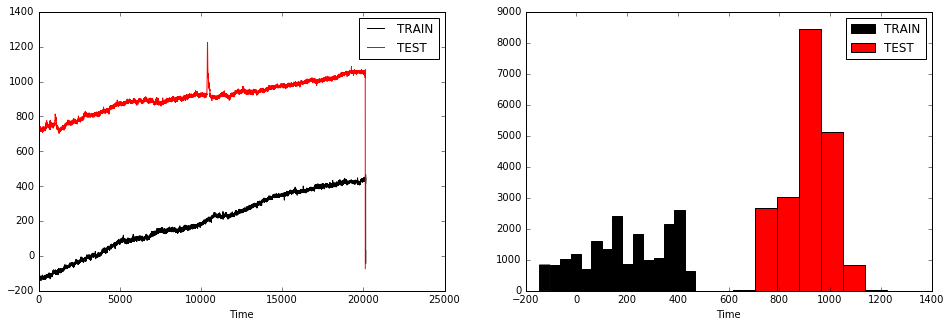
\includegraphics[width = \textwidth]{field4_plots.png}
   \caption{Значения field 4 в тренировочной и тестовой выборках} \label{img:field4_plots}    
  \end{minipage}  
   \hfill
  \begin{minipage}[h]{0.49\linewidth}
      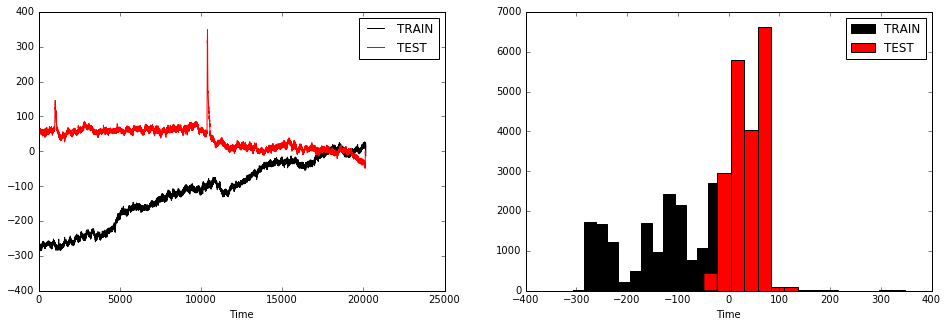
\includegraphics[width = \textwidth]{field19_plots.png}
    \caption{Значения field 19 в тренировочной и тестовой выборках} \label{img:field19_plots}    
  \end{minipage}  
 \end{center}
\end{figure}

\section{Стандартные методы} 
В качестве стандартных методов классификации были использованы линейный дискриминантный анализ (LDA), логистическая регрессия (LogRegression), метод градиентного бустинга (библиотека XGBoost) и Linear SVC (Support Vector Classification). Для рассматриваемых методов данные преобразовывались к значениям от 0 до 1 следующим образом: для вектора $x=\{x_1,~x_2,~\ldots,~x_n\}$ преобразованным вектором назовем $x'=\{x'_1,~x'_2,~\ldots,~x'_n\}$, где $$x'_i = \frac{x_i - \min\{x\}}{\max\{x\} - min\{x\}}$$.
Затем, на вход классификаторам подавались первые три главные компоненты, полученные методом аппроксимации данных principal component analysis (PCA).

Наилучший результат с помощью этих методов удалось получить, используя LDA и логистическую регрессию.

Численное сравнение результатов методов описано в разделе \ref{compute_part:method_compare}.

\section{Классификация с помощью моделей временной иерархической памяти}
С помощью алгоритмов пакета nupic, реализованного на языке Python (2.7), были построены две модели HTM: 
\begin{enumerate}
\item NontemporalClassification;
\item Модель на основе комбинирования MultiStep моделей.
\end{enumerate}
Остановимся на каждой из них подробнее.

\subsection{Модель NontemporalClassification}
Метка Nontemporal в названии модели предполагает, что при такой классификации обученная сеть не запоминает последовательности в данных, а классифицирует каждое наблюдение отдельно. Это свойство делает метод похожим на стандартные методы классификации.

\subsection{Ансамбль MultiStep моделей}
Одним из главных аспектов HTM является работа с непрерывными временными данными. Она основывается на способности Temporal Pooler выучивать временные шаблоны в данных. Поэтому рассмотрим следующую модель:
\begin{itemize}
\item Разделяем тренировучную выборку на имеющиеся классы.
\item Обучаем модель для каждого класса. Для этого внутри классов для каждого из признаков <<field i>> обучается модель предсказания будущих значения; модель строится не только по предыдущим значениям фиксированного признака, но по всех значениям признаков на предыдущих временных отсчетах.
\item Подаем данные из тестовой выборки в каждую из моделей класса (в нашем случае их три).
\item Вычисляем ошибки в предсказаниях на тестовой выборке. 
\item Присваиваем наблюдению тот класс, на котором была достигнута минимальная из посчитанных на предыдущем шаге ошибок.
\end{itemize} 

Проблема модели заключается в больших временных затратах на обучение: имея 3 класса и 24 признака, нужно обучить 72 модели. Одним из вариантов решения является разделение всех признаков на группы коррелирующих между собой и выбор из каждой группы одного представителя, наиболее сильно влияющего на целевую переменную с метками класса.

\section{Сравнение методов}\label{compute_part:method_compare}
В таблице \ref{tbl:results_compare} представлены результаты, полученные с помощью рассматриваемых методов. В качестве мер ошибки использованы мера точности (Accuracy) и F-measure. По результатам видно, что на тестовой выборке ошибка предсказания для модели NontemporalClasification временной иерархической памяти пренебрежимо мала, и точность предсказания значительно превосходит точность стандартных методов классификации для анализировавшихся данных.
 
\begin{table}[h!]
\caption{Сравнение методов классификации.} \label{tbl:results_compare} 
 \begin{center}
  \begin{tabular}{|c|c|c|c|}
	\hline  & Регуляризация & Accuracy & F-measure \\ 
	\hline LDA & $\lambda = 0.2$ & 0.87 & 0.868 \\ 
	\hline Linear SVC (C = 1.0)  & --- & 0.756 & 0.747  \\
	\hline LogRegression  & ---  & 0.877 & 0.88 \\
	\hline XGBoost  &  $\lambda = 0.75$   & 0.787 & 0.79 \\
	\hline NontemporalClassification & --- & 0.999 & 0.999 \\
	\hline 
  \end{tabular} 
 \end{center}
\end{table}


\bibliographystyle{acm}
\bibliography{ivanova_pm_cw_16}
\end{document}